\documentclass[tikz,border=2pt]{standalone}
\usepackage{amsmath}
\usetikzlibrary{arrows.meta}
\begin{document}
% Prisoner's Dilemma (Mum M / Fink F) drawn as a sequence: if player 2 does not observe player 1's
% choice, her two nodes form one information set, so her strategy is a single action and the game
% is the static game with profile set S_1 x S_2, i.e. the 2x2 payoff matrix on the right.
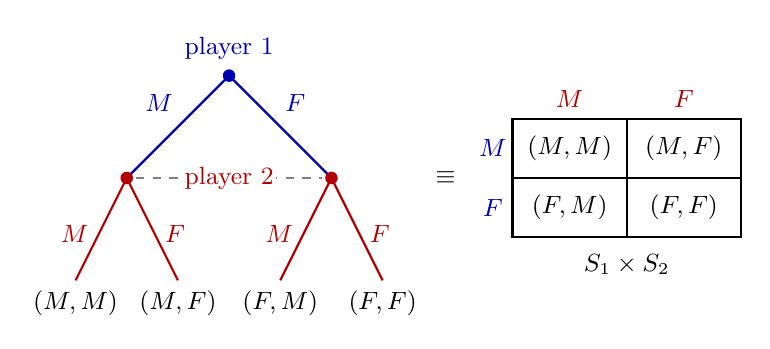
\begin{tikzpicture}[font=\small, >={Latex[length=2mm]},
    dec/.style={circle, fill, inner sep=1.6pt}]
  % tree
  \draw[thick, blue!70!black] (2.0,0) -- node[above left, pos=0.45] {$M$} (0.7,-1.3);
  \draw[thick, blue!70!black] (2.0,0) -- node[above right, pos=0.45] {$F$} (3.3,-1.3);
  \foreach \px/\a in {0.7/M, 3.3/F} {
    \draw[thick, red!70!black] (\px,-1.3) -- node[left, pos=0.55] {$M$} (\px-0.65,-2.6);
    \draw[thick, red!70!black] (\px,-1.3) -- node[right, pos=0.55] {$F$} (\px+0.65,-2.6);
    \node[anchor=north, inner sep=2pt] at (\px-0.65,-2.65) {$(\a,M)$};
    \node[anchor=north, inner sep=2pt] at (\px+0.65,-2.65) {$(\a,F)$};
  }
  \node[dec, blue!70!black, label={[blue!70!black]above:player 1}] at (2.0,0) {};
  \node[dec, red!70!black] at (0.7,-1.3) {};
  \node[dec, red!70!black] at (3.3,-1.3) {};
  \draw[dashed, thick, gray] (0.82,-1.3) -- (3.18,-1.3);
  \node[red!70!black, fill=white, inner sep=1pt] at (2.0,-1.3) {player 2};
  % equivalent matrix
  \node at (4.75,-1.3) {$\equiv$};
  \begin{scope}[xshift=5.6cm, yshift=-1.3cm]
    \def\w{1.45} \def\h{0.75}
    \draw[thick] (0,-\h) rectangle (2*\w,\h);
    \draw[thick] (\w,-\h) -- (\w,\h);
    \draw[thick] (0,0) -- (2*\w,0);
    \node[red!70!black] at (0.5*\w,\h+0.25) {$M$};
    \node[red!70!black] at (1.5*\w,\h+0.25) {$F$};
    \node[blue!70!black] at (-0.25,0.5*\h) {$M$};
    \node[blue!70!black] at (-0.25,-0.5*\h) {$F$};
    \node at (0.5*\w,0.5*\h) {$(M,M)$};
    \node at (1.5*\w,0.5*\h) {$(M,F)$};
    \node at (0.5*\w,-0.5*\h) {$(F,M)$};
    \node at (1.5*\w,-0.5*\h) {$(F,F)$};
    \node[anchor=north] at (\w,-\h-0.1) {$S_1\times S_2$};
  \end{scope}
\end{tikzpicture}
\end{document}
